
\begin{document}
\abstract{Balanced Scorecard y Business model canvas son técnicas de análisis empresarial . Ambas técnicas son útiles para mejorar el desempeño organizacional. Pero sus aplicaciones difieren. Ambos se pueden usar junto con los indicadores clave de rendimiento para monitorear y mejorar el rendimiento de la organización. Vamos a entender tanto la técnica en detalle.}

 Abstract\\
Balanced Scorecard and Business model canvas are business analysis techniques. Both techniques are useful to improve organizational performance. But their applications differ. Both can be used together with the key performance indicators to monitor and improve the performance of the organization. We will understand both the technique and the detail.
\newpage

\section{Introducción}
En la actualidad, las tecnologías de la información han automatizado los procesos de carácter típicamente repetitivo o administrativo, haciendo uso de lo que se denomina sistemas de información operacionales. Dichos sistemas resuelven las necesidades de funcionamiento de la empresa, donde sus principales características son la actualización y el tiempo de respuesta. 

Las necesidades informacionales (necesidades de funcionamiento de la empresa), son aquellas que tienen por objeto obtener la información necesaria, que sirva de base para la toma de decisiones tanto a escala estratégica como táctica. Estas necesidades se basan en gran medida en el análisis de un número ingente de datos, en el que es tan importante el obtener un valor muy detallado de negocio como el valor totalizado para el mismo. Así también, es fundamental la visión histórica de todas las variables analizadas, y el análisis de los datos del entorno. 

Cualquier actividad que realiza la empresa está reflejada de forma minuciosa en sus bases de datos, por lo tanto, esto puede derivarnos en diferentes problemas de tipo informacional. En primer lugar, al realizar consultas masivas de información, se puede ver perjudicado el nivel de servicio del resto de sistemas, dado que las consultas de las que estamos hablando, suelen ser bastante costosas en recursos. Dichas necesidades se ven insatisfechas por la limitada flexibilidad a la hora de navegar por la información y a su inconsistencia debido a la falta de una visión global En esta situación, el siguiente paso evolutivo ha venido siendo la generación de un entorno gemelo del operativo, que se ha denominado comúnmente Centro de Información. 

\begin{center}
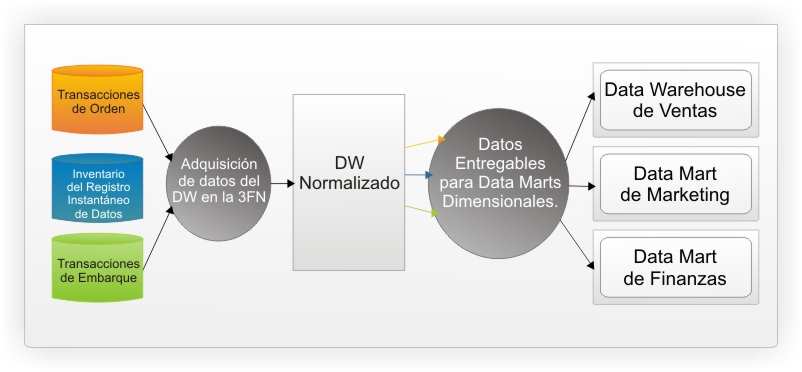
\includegraphics[width=16cm]{./Imagenes/image003}
\end{center}


\newpage


\section{METODOLOGÍA INMON VS METODOLOGÍA KIMBALL}


\section{METODOLOGÍA INMON}
\section{Historia:}
1990 publica Building the Data Warehouse y en 2002 mejora su libro y define una arquitectura como una colección de fuentes dispares en almacenes de datos y variantes en el tiempo.
\section{Concepto}
Bill Inmon es considerado el padre del concepto Data Warehouse, el menciona que un Data Warehouse debe cumplir con las siguientes \section{características:}
•	Dirigido a un área. Datos sobre un área específica en lugar de operaciones de la compañía\\
•	Integrado. Unión de diferentes fuentes de datos de manera coherente.\\
•	Variable en el tiempo. Todos los datos pertenecen a un periodo de tiempo determinado.\\
•	No volátil. Los datos no son eliminados.\\
La metodología que Bill Inmon propone es iterativa la cual sigue un esquema contrario al clásico de desarrollo de sistemas ya que lo primero con lo que se trabaja son datos, estos se integran para ser probados y programar de acuerdo con ellos para analizar los resultados y de esta manera comprender los requerimientos. 
La información ha de estar a los máximos niveles de detalle. Los Dw departamentales o Data Marts son tratados como subconjuntos de este Dw corporativo, que son construidos para cubrir las necesidades individuales de análisis de cada departamento, y siempre a partir de este Dw Central (del que también se pueden construir los ODS (Operacional Data Stores) o similares).\\
\begin{center}
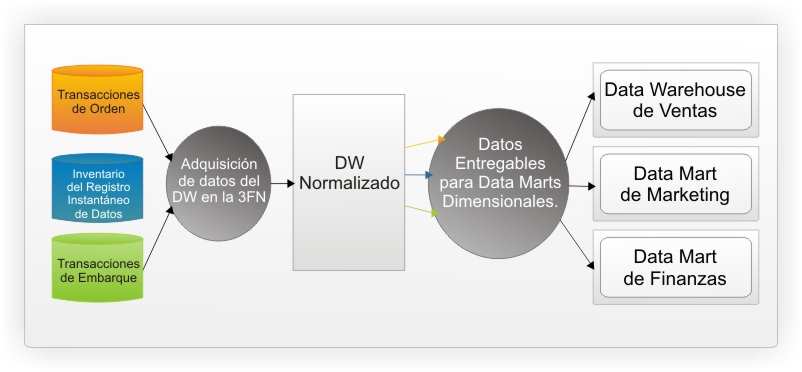
\includegraphics[width=16cm]{./Imagenes/image003}
\end{center}
 
El enfoque Inmon también se referencia normalmente como Top-Down. Los datos son extraídos de los sistemas operacionales por los procesos ETL y cargados en las áreas de stage, donde son validados y consolidados en el DW corporativo, donde además existen los llamados metadatos que documentan de una forma clara y precisa el contenido del DW. Una vez realizado este proceso, los procesos de refresco de los Data Marts departamentales obtienen la información de él, y con las consiguientes transformaciones, organizan los datos en las estructuras particulares requeridas por cada uno de ellos, refrescando su contenido.\\
Dentro de esta metodología se menciona que la construcción de toda la arquitectura de un Data Warehouse toma bastante tiempo, puesto que su desarrollo inicial está relacionado con necesidades genéricas empresariales, a lo largo del tiempo este tipo de necesidades son cubiertas por el Data Warehouse para más personas por lo que la demanda del uso del Data Warehouse aumenta y esto hace que el performance se vea afectado. Es por esto que al llegar a este punto se comienzan a construir segmentos del Data Warehouse que se alimentaran del Data Warehouse y que permitirán tener la información almacenada de manera que esta vaya dirigida a departamentos, con esto se logra disminuir la demanda sobre el Data Warehouse debido a que por ejemplo para estos momentos en lugar de tener a 100 usuarios requiriendo de manera directa los servicios del Data Warehouse tendré 5 departamentos.

\section{Data Warehouse}
Un data warehouse es donde se concentrar todos los datos con un diseño especial para explotar información. Se componen por fragmentos derivados del DATA WHAREHOUSE conocidos como DATAMARTS.
Normalmente, un data warehouse se aloja en un servidor corporativo o cada vez más, en la nube. Los datos de diferentes aplicaciones de procesamiento de transacciones Online (OLTP) y otras fuentes se extraen selectivamente para su uso por aplicaciones analíticas y de consultas por usuarios.
Data Warehouse es una arquitectura de almacenamiento de datos que permite a los ejecutivos de negocios organizar, comprender y utilizar sus datos para tomar decisiones estratégicas. Un data warehouse es una arquitectura conocida ya en muchas empresas modernas.
 
 \begin{center}
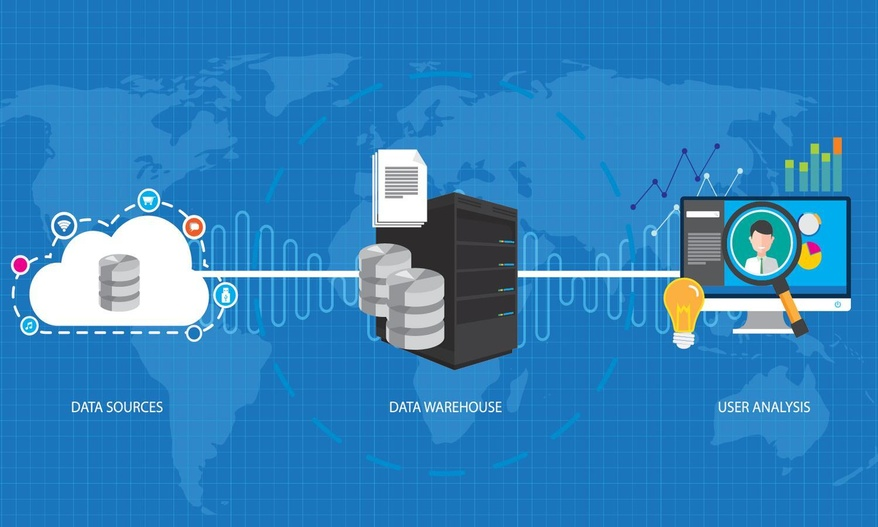
\includegraphics[width=12cm]{./Imagenes/image005}
\end{center}

El DATA WAREHOUSE no es software, mucho menos una marca o una sola base de datos, en general podemos abstraernos de los modelos lógicos y físicos de la base de datos.
 
\section{Estructuras de un Data Warehouse}
La arquitectura de un data warehouse puede ser dividida en tres estructuras simplificadas: básica, básica con un área de ensayo y básica con área de ensayo y data Marts.\\
•	Con una estructura básica, sistemas operativos y archivos planos proporcionan datos en bruto que se almacenan junto con metadatos. Los usuarios finales pueden acceder a ellos para su análisis, generación de informes y minería.\\
•	Al añadir un área de ensayo que se puede colocar entre las fuentes de datos y el almacén, ésta proporciona un lugar donde los datos se pueden limpiar antes de entrar en el almacén. Es posible personalizar la arquitectura del almacén para diferentes grupos dentro de la organización.\\
•	Se puede hacer agregando data Marts, que son sistemas diseñados para una línea de negocio en particular. Se pueden tener data Marts separados para ventas, inventario y compras, por ejemplo, y los usuarios finales pueden acceder a datos de uno o de todos los data Marts del departamento.\\
\begin{center}
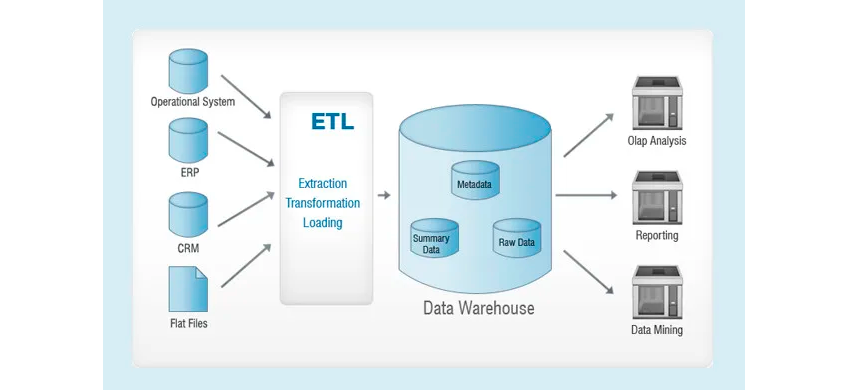
\includegraphics[width=12cm]{./Imagenes/image007}
\end{center}
 
\section{Propósitos del Data Warehouse}
•	Es enfocado a toda la empresa\\
•	Debe ajustarse a los cambios\\
•	Preparado para carga masiva de datos en un pequeño lapso de tiempo○\\
•	Diseñado para el análisis de información\\
•	No es conveniente que el data warehouse conviva en el mismo\\ ambiente que nuestros sistemas transaccionales como: ERP.\\
•	La naturaleza del data warehouse debe ser multipropósito\\

\section{Algunas Metodologías}

\begin{center}
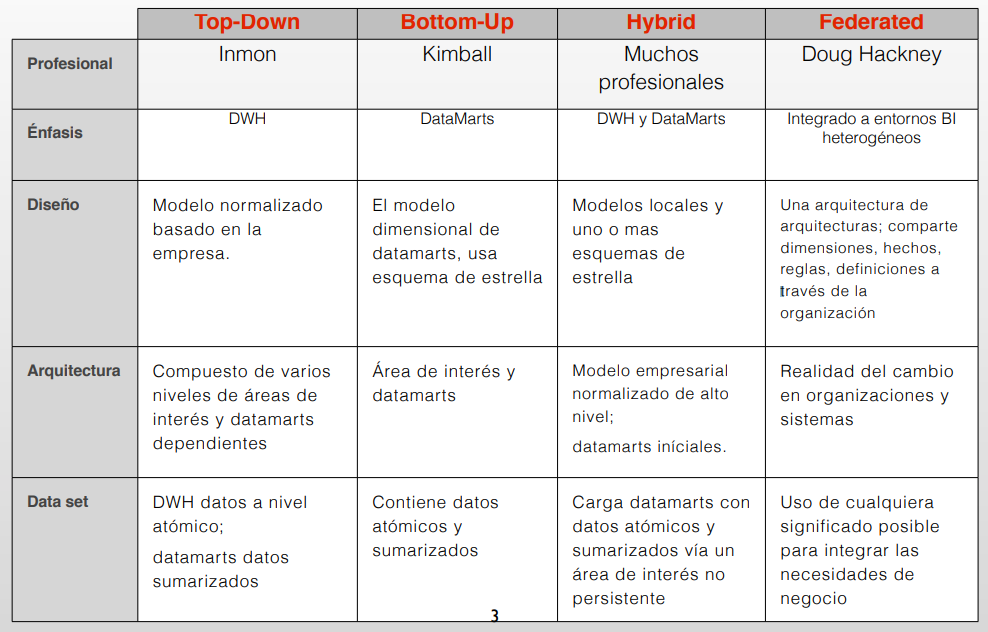
\includegraphics[width=16cm]{./Imagenes/image009}
\end{center}
\newpage
\section{METODOLOGÍA DE KIMBALL}
La Metodología Kimball, es una metodología empleada para la construcción de un almacén de datos (data warehouse, DW) que no es más que, una colección de datos orientada a un determinado ámbito (empresa, organización, etc.), integrado, no volátil y variable en el tiempo, que ayuda a la toma de decisiones en la entidad en la que se utiliza.\\
La metodología se basa en lo que Kimball denomina Ciclo de Vida Dimensional del Negocio (Business Dimensional Lifecycle). Este ciclo de vida del proyecto de DW, está basado en cuatro principios básicos:\\
•	Centrarse en el negocio\\
•	Construir una infraestructura de información adecuada\\
•	Realizar entregas en incrementos significativos (este principio consiste en crear el almacén de datos (DW) en incrementos entregables en plazos de 6 a 12 meses, en este punto, la metodología se parece a las metodologías ágiles de construcción de software)\\
•	Ofrecer la solución completa (En este se punto proporcionan todos los elementos necesarios para entregar valor a los usuarios de negocios, para esto ya se debe tener un almacén de datos bien diseñado, se deberán entregar herramientas de consulta ad hoc, aplicaciones para informes y análisis avanzado, capacitación, soporte, sitio web y documentación).\\
La construcción de una solución de DW/BI (Datawarehouse/Business Intelligence) es sumamente compleja, y Kimball nos propone una metodología que nos ayuda a simplificar esa complejidad. Las tareas de esta metodología (ciclo de vida) se describen a continuación:
.\\\\\

\begin{center}
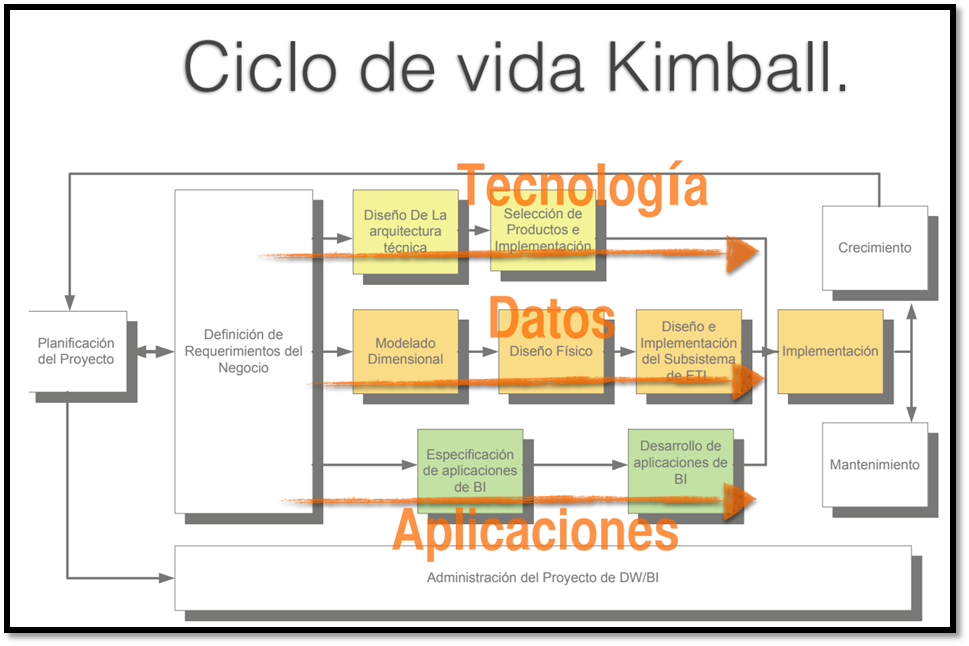
\includegraphics[width=15cm]{./Imagenes/image011}
\end{center}

\section{1.1.PLANIFICACIÓN DEL PROYECTO}\\
En este proceso se determina el propósito del proyecto de DW/BI,
sus objetivos específicos y el alcance de este, los principales riesgos
y una aproximación inicial a las necesidades de información.\\

Esta tarea incluye las siguientes acciones típicas de un plan de proyecto:\\
	Definir el alcance (entender los requerimientos del negocio).\\
	Identificar las tareas\\
	Programar las tareas\\
	Planificar el uso de los recursos.\\
	Asignar la carga de trabajo a los recursos\\
	Elaboración de un documento final que representa un plan del proyecto.\\
Además, en esta parte definimos cómo realizar la administración o gestión de esta subfase que es todo un proyecto en sí mismo, con las siguientes actividades:\\
•	Monitoreo del estado de los procesos y actividades.\\
•	Rastreo de problemas\\
•	Desarrollo de un plan de comunicación comprensiva que direccione la empresa y las áreas de TI\\
.\\\\
\section{DEFINICIÓN DE REQUERIMIENTOS DEL NEGOCIO}
CLa definición de requerimientos es un proceso de entrevistar al personal de negocio y técnico, aunque siempre conviene, tener un poco de preparación previa. En esta tarea, se debe aprender sobre el negocio, los competidores, la industria y los clientes de este. Se debe dar una revisión a todos los informes posibles de la organización; rastrear los documentos de estrategia interna; entrevistar a los empleados, analizar lo que se dice en la prensa acerca de la organización, la competencia y la industria y se deben conocer los términos y la terminología del negocio.\\

Se sugiere entrevistar al personal que se encuentra en los cuatro grupos que se mencionan a continuación:\\
•	El directivo responsable de tomar las decisiones estratégicas.\\
•	Los administradores intermedios y de negocio responsables de explorar alternativas estratégicas y aplicar decisiones\\
•	El personal de sistemas, si existe (estas son las personas que realmente saben qué tipos de problemas informáticos y de datos existen en la organización)\\
•	El personal que se entrevista por razones políticas.\\
Entre las tareas antes descritas, existe una flecha bidireccional, esto indica que los requerimientos del negocio son el soporte inicial de las tareas subsiguientes, también tiene influencia en el plan de proyecto.\\
Si avanzamos por el camino central del diagraman, encontramos las tareas asociadas al área de Datos, en esta, diseñaremos e implementaremos el modelo dimensional, y desarrollaremos el subsistema de Extracción, Transformación y Carga (Extract, Transformation, and Load - ETL) para cargar el DW. Las tareas pertenecientes al área se describen a continuación:\\
Si avanzamos por el camino central del diagraman, encontramos las tareas asociadas al área de Datos, en esta, diseñaremos e implementaremos el modelo dimensional, y desarrollaremos el subsistema de Extracción, Transformación y Carga (Extract, Transformation, and Load - ETL) para cargar el DW. Las tareas pertenecientes al área se describen a continuación.\\
\\\\
\section{MODELADO DIMENSIONAL}
Es un proceso dinámico y altamente iterativo. Comienza con un modelo dimensional de alto nivel obtenido a partir de los procesos priorizados y descritos en la tarea anterior, y El proceso iterativo consiste en cuatro pasos:\\
a)	Elegir el proceso de negocio: que consiste en, elegir el área a modelizar. Esta es una decisión de la dirección, y depende fundamentalmente del análisis de requerimientos y de los temas analíticos anotados en la etapa anterior.\\
b)	Establecer el nivel de granularidad: La granularidad significa especificar el nivel de detalle. La elección de la granularidad depende de los requerimientos del negocio y lo que es posible a partir de los datos actuales. La sugerencia general es comenzar a diseñar el DW al mayor nivel de detalle posible, ya que se podrían realizar agrupamientos posteriores, al nivel deseado.\\
c)	Elegir las dimensiones: Las dimensiones surgen naturalmente de las discusiones del equipo, y facilitadas por la elección del nivel de granularidad y de la matriz de procesos/dimensiones (que se realiza en la tarea 4.2) Las tablas de dimensiones tienen un conjunto de atributos (generalmente textuales) que brindan una perspectiva o forma de análisis sobre una medida en una tabla hechos. Una forma de identificar las tablas de dimensiones es que sus atributos son posibles candidatos para ser encabezado en los informes, tablas pivot, cubos, o cualquier forma de visualización, unidimensional o multidimensional.\\
d)	Identificar medidas y las tablas de hechos: Este paso, consiste en identificar las medidas que surgen de los procesos de negocios. Una medida es un atributo (campo) de una tabla que se desea analizar, sumando o agrupando sus datos y usando los criterios de corte conocidos como dimensiones. Las medidas habitualmente se vinculan con el nivel de granularidad del punto 2, y se encuentran en tablas que denominamos tablas de hechos (fact en inglés). Cada tabla de hechos tiene como atributos una o más medidas de un proceso organizacional, de acuerdo a los requerimientos. Un registro contiene una medida expresada en números, como ser cantidad, tiempo, dinero, etc., sobre la cual se desea realizar una operación de agregación (promedio, conteo, suma, etc.) en función de una o más dimensiones. La granularidad, en este punto, es el nivel de detalle que posee cada registro de una tabla de hechos.\\
\section{DISEÑO FÍSICO}
En esta tarea, se contestan las siguientes preguntas:\\
o	¿Cómo puede determinar cuán grande será el sistema de DW/BI?
o	¿Cuáles son los factores de uso que llevarán a una configuración más grande y compleja?\\
o	¿Cómo se debe configurar el sistema?\\
o	¿Cuánta memoria y servidores se necesitan? ¿Qué tipo de almacenamiento y procesadores?\\
o	¿Cómo instalar el software en los servidores de desarrollo, prueba y producción?\\
o	¿Qué necesitan instalar los diferentes miembros del equipo de DW/BI en sus estaciones de trabajo?\\
o	¿Cómo convertir el modelo de datos lógico en un modelo de datos físicos en la base de datos relacional?\\
o	¿Cómo conseguir un plan de indexación inicial?\\
o	¿Debe usarse la partición en las tablas relacionales?\\



\begin{center}
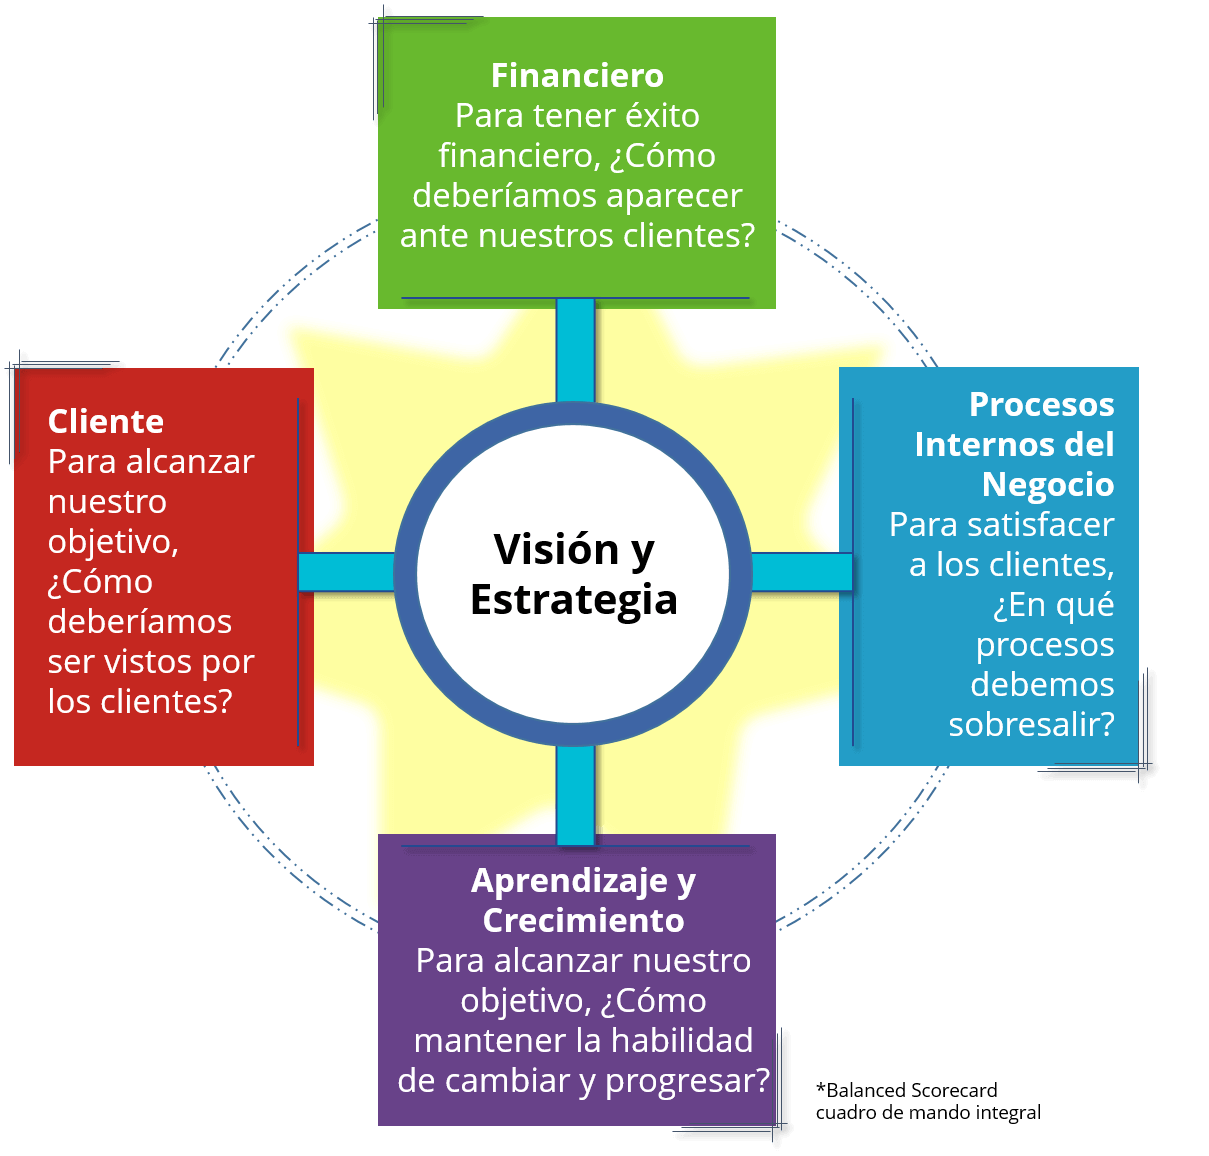
\includegraphics[width=15cm]{./Imagenes/imagen2}
\end{center}

\section{DISEÑO E IMPLEMENTACIÓN DEL SUBSISTEMA DE EXTRACCIÓN, TRANSFORMACIÓN Y CARGA (ETL)}
\item{El subsistema de Extracción, Transformación y Carga (ETL) es la base sobre la cual se alimenta el Data warehouse. Si se diseña adecuadamente, puede extraer los datos de los sistemas de origen de datos, aplicar diferentes reglas para aumentar la calidad y consistencia de estos, consolidar la información proveniente de distintos sistemas, y finalmente cargar (grabar) la información en el DW en un formato acorde para la utilización por parte de las herramientas de análisis.}



\section{IMPLEMENTACIÓN}
\item{La implementación representa la convergencia de la tecnología, los datos y las aplicaciones de usuarios finales accesible desde el escritorio del usuario del negocio. Existen varios factores extras que aseguran el correcto funcionamiento de todas estas piezas, entre ellos se encuentran la capacitación, el soporte técnico, la comunicación y las estrategias de feedback.}



\section{MANTENIMIENTO Y CRECIMIENTO DEL DATA WAREHOUSE}
\item{
Para administrar el entorno del Data Warehouse existente es importante enfocarse en los usuarios de negocio, los cuales son el motivo de su existencia, además de gestionar adecuadamente las operaciones del Data Warehouse, medir y proyectar su éxito y comunicarse constantemente con los usuarios para establecer un flujo de retroalimentación, En esto consiste el Mantenimiento. Finalmente, es importante sentar las bases para el crecimiento y evolución del Data Warehouse en donde el aspecto clave es manejar el crecimiento y evolución de forma iterativa utilizando el Ciclo de Vida propuesto, y establecer las oportunidades de crecimiento y evolución en orden por nivel prioridad.
Si avanzamos por el camino inferior del diagraman, encontramos las tareas asociadas al área Aplicaciones de Inteligencia de Negocios, en esta ruta se encuentran tareas en las que diseñamos y desarrollamos las aplicaciones de negocios para los usuarios finales. Las tareas pertenecientes al área se describen a continuación:

}

\section{ESPECIFICACIÓN DE APLICACIONES DE BI}
\item{
En esta tarea se proporciona, a una gran comunidad de usuarios una forma más estructurada y por lo tanto, más fácil, de acceder al almacén de datos. Se proporciona este acceso estructurado a través de lo que llamamos, aplicaciones de inteligencia de negocios (Business Intelligence Aplications). Las aplicaciones de BI son la cara visible de la inteligencia de negocios: los informes y aplicaciones de análisis proporcionan información útil a los usuarios. Las aplicaciones de BI incluyen un amplio espectro de tipos de informes y herramientas de análisis, que van desde informes simples de formato fijo, a sofisticadas aplicaciones analíticas que usan complejos algoritmos e información del dominio. Kimball divide a estas aplicaciones en dos categorías basadas en el nivel de sofisticación, y les llama:
a)	Informes estándar: son informes relativamente simples, de formato predefinido, y parámetros de consulta fijos, proporcionan a los usuarios un conjunto básico de información acerca de lo que está sucediendo en un área determinada de la empresa y se utilizan día a día.
b)	Aplicaciones analíticas: Son más complejas que los informes estándar. Estas aplicaciones pueden incluir algoritmos y modelos de minería de datos, que ayudan a identificar oportunidades o cuestiones subyacentes en los datos, y el usuario puede pedir cambios en los sistemas transaccionales basándose en los conocimientos obtenidos del uso de la aplicación de BI. Algunas aplicaciones analíticas comunes incluyen:\\

•	Análisis de la eficacia de la promoción\\
•	Análisis de rutas de acceso en un sitio Web\\
•	Análisis de afinidad de programas\\
•	Planificación del espacio en espacios comerciales\\\\
•	Detección de fraudes\\
•	Administración y manejo de categorías de productos\\
Por último, en el camino superior, encontramos las tareas asociadas al área Tecnología en esta ruta, se encuentran las tareas relacionadas con software específico, por ejemplo, Microsoft SQL Analysis Services, etc. Las tareas pertenecientes al área se describen a continuación
}
\begin{center}
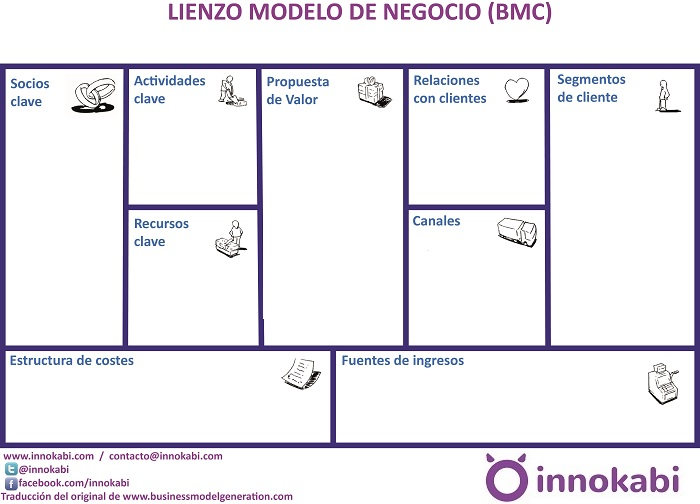
\includegraphics[width=15cm]{./Imagenes/imagen4}
\end{center}

\section{DISEÑO DE LA ARQUITECTURA TÉCNICA}
\item{El área de arquitectura técnica cubre los procesos y herramientas que se aplican a los datos. En el área técnica existen dos conjuntos que tienen distintos requerimientos, brindan sus propios servicios y componentes de almacenaje de datos, por lo que se consideran cada uno aparte: El back room (habitación trasera) y el front room (habitación frontal). El back room es el responsable de la obtención y preparación de los datos, por lo que también se conoce como adquisición de datos y el front room es responsable de entregar los datos a la comunidad de usuario y también se le conoce como acceso de datos.
}

\section{COMPARATIVA ENTRE INMON Y KIMBALL}
\item{
Poco precisa, no sirve para operativa concreta.\\
Se debe complementar con mapa de procesos detallados.\\
Por ser tan novedosa puede hacernos creer que completando el lienzo ya tenemos el modelo resuelto}

\begin{center}
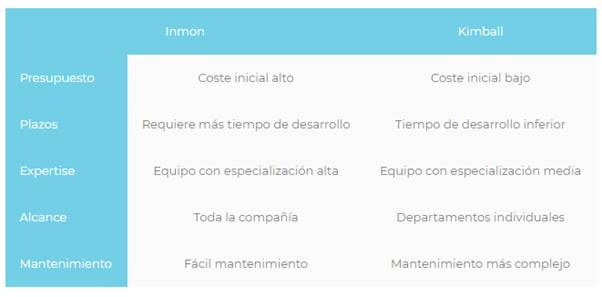
\includegraphics[width=15cm]{./Imagenes/image014}
\end{center}

\begin{center}
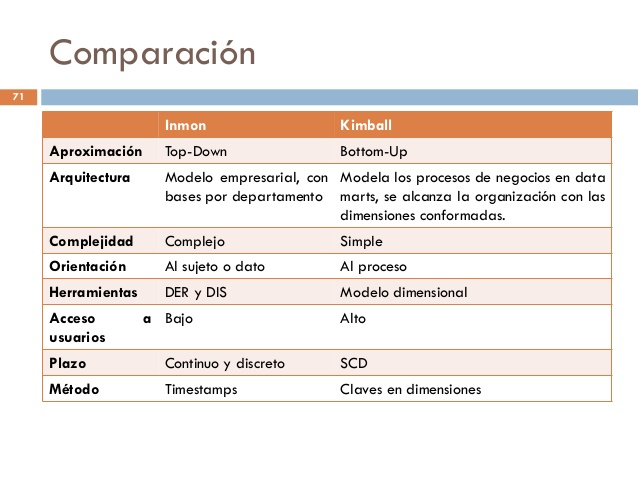
\includegraphics[width=15cm]{./Imagenes/image015}
\end{center}

\begin{center}
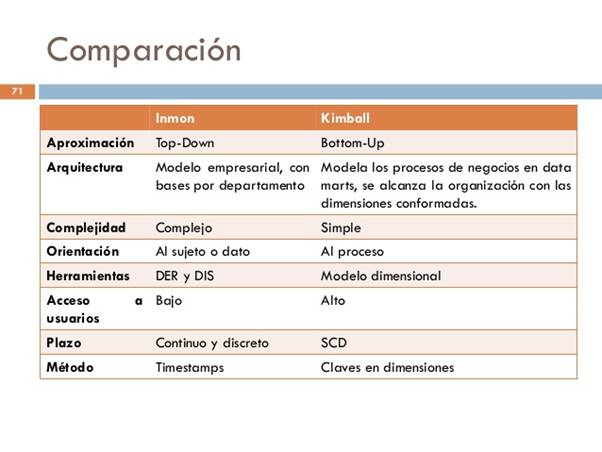
\includegraphics[width=15cm]{./Imagenes/image016}
\end{center}

\begin{center}
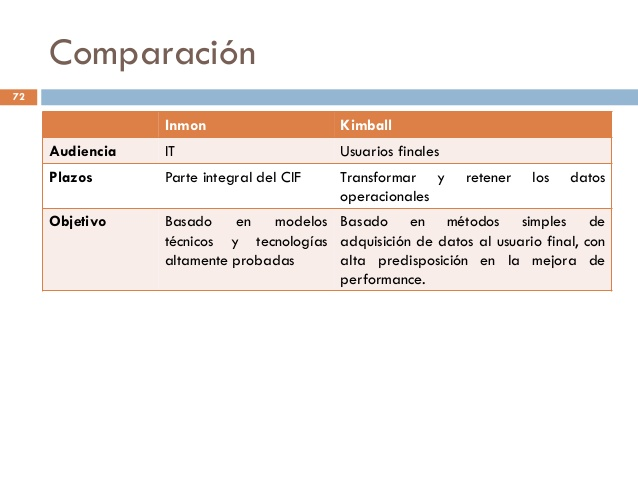
\includegraphics[width=15cm]{./Imagenes/image017}
\end{center}
\begin{center}
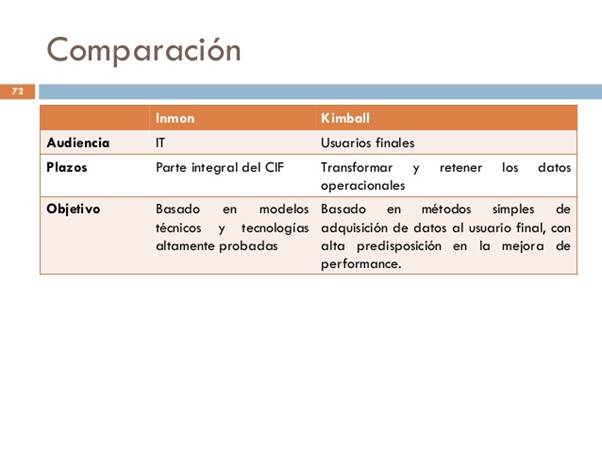
\includegraphics[width=15cm]{./Imagenes/image018}
\end{center}

\newpage
% Bibliografía.
%-----------------------------------------------------------------
\begin{thebibliography}{99}
https://www.isotools.org/2015/02/23/que-es-el-balanced-scorecard-conoce-su-funcionamiento-y-ventajas/\\
https://economipedia.com/definiciones/modelo-canvas.html\\
http://www.infoviews.com.mx/Bitam/ScoreCard/]\\
https://josefacchin.com/modelo-canvas-de-negocio/\\
https://www.adaptiveus.com/balanced-scorecard-vs-business-model-canvas/\\
https://innokabi.com/canvas-de-modelo-de-negocio/\\


\bibitem{Cd94} Autor, \emph{Título}, Revista/Editor, (año)

\end{thebibliography}

\end{document}

